\section{Dependencia e independencia lineal}

\begin{defi}
	\label{def: ld y li}
Sea $V$ un $F-$espacio vectorial. Decimos que $S \subseteq V$
es \textbf{linealmente dependiente} si existe un número
finito de vectores distintos entre si $x_{1}, \ldots , x_{n} \in S$
y escalares $a_{1}, \ldots , a_{n} \in F$ no todos cero
\marginnote{Abreviamos los términos linealmente dependiente
(resp. independiente) como \textbf{l.d.} (resp. \textbf{l.i.}).}
tales que 
\[
\sum_{i=1}^{n} a_{i}x_{i} = \hat{0}.
\]
Si $S$ no es linealmente dependiente, diremos que es
\textbf{linealmente independiente}.
\end{defi}

En la definición \ref{def: ld y li}
pedimos
\begin{itemize}
	\item que los vectores $x_{i}$ sea distintos entre sí, y
	\item que al menos uno de los escalares $a_{i}$ sea no cero,
\end{itemize}
pues las igualdades
	\[
	1_{F} x + (-1_{F}) x = x - x = \hat{0}
	\]
	y
	\[
	0_{F} x = \hat{0},
	\]
	son ciertas \textit{para todo $x \in V$}, ¡no las vamos a usar
	para definir un nuevo concepto!
	
Si un conjunto finito $S = \{ x_{1}, \ldots , x_{n} \}$
es l.d.(resp. l.i.), acostumbramos decir que los vectores
$x_{1}, \ldots , x_{n}$ son l.d. (resp. l.i.).


\hlgray{Ejercicio:}
Niegue la definición de dependencia lineal dada en 
\ref{def: ld y li} para obtener la definición de independencia lineal.

\begin{ejem}
\begin{itemize}
	\item Por vacuidad, el conjunto vacío es linealmente independiente
	\item Todo subconjunto de $S$ que que contenga al cero es
	linealmente dependiente
\end{itemize}
\diam

\end{ejem}
\hlgray{Ejercicio:} demuestre a detalle los puntos del ejemplo anterior.

\hlgray{Ejercicio:} demuestre que, dados $S \subseteq T \subseteq V$,
\begin{itemize}
	\item si $T$ es l.i., entonces $S$ es l.i.
	\item si $S$ es l.d., entonces $T$ es l.d. 
\end{itemize}

\hlgray{Ejercicio:} demuestre que 
si $x_{1}, \ldots , x_{n}$ distintos entre sí son l.i. y
$a_{1} x_{1} + \cdots + a_{n} x_{n} = \hat{0}$, entonces todos
los escalares $a_{i}$ son iguales a cero.


\begin{prop}
	\label{prop: ld equiv fried y hugo}
\marginnote{El enunciado dado en la proposición 
\ref{prop: ld equiv fried y hugo} es
la definición de dependencia lineal manejada por Hugo Rincón (REF).}
$S \subseteq V$ es linealmente dependiente si y sólo si 
existe $x \in S$ tal que $x \in \langle S - \{ x \} \rangle$.
\end{prop}
\noindent
\textbf{Demostración.}
\begin{itemize}
	\item[$\Rightarrow$]] Sean $x_{1},\ldots , x_{n} \in S$
	distintos entre sí y $a_{1}, \ldots , a_{n}$ escalares no cero 
	tales que $\sum_{i=1}^{n} a_{i}x_{i} = \hat{0}$.
	Sin pérdida de generalidad, supongamos que 
	$a_{1} \neq 0$. Entonces,
	\[
	a_{1}x_{1} = - \sum_{i=2}^{n} a_{i}x_{i} \in 
	\langle S - \{ x_{1} \} \rangle,
	\]
	luego, $x_{1} \in \langle S -\{ x_{1} \} \rangle$.
	\item[$\Leftarrow$]] Sea $x \in S$ tal que 
	$x \in \langle S - \{ x \} \rangle$. Sean pues
	$x_{1}, \ldots ,x_{n} \in S - \{ x \}$ distintos
	entre si 
	tales que $x = \sum_{i = 1}^{n} a_{i}x_{i}$. Restando $x$
	de ambos lados de la igualdad llegamos a que
	\[
	\hat{0} = \sum_{i = 1}^{n} a_{i}x_{i} - x
	= \sum_{i = 1}^{n} a_{i}x_{i} + (-1_{F}) x.
	\]
	(c.f. prop REF). Como $-1_{F} \neq 0_{F}$, esta última
	igualdad muestra que $S$ es linealmente dependiente.
	
\end{itemize}

\QEDB
\vspace{0.2cm}

\begin{prop}
	\label{prop: singulete x l.i. sii x no cero}
Un singulete $\{ x \} \subseteq V$ es linealmente independiente en $V$
si y sólo si $x \neq \hat{0}$.
\end{prop}
\noindent
\textbf{Demostración.}
En efecto, según la proposición
\ref{prop: ld equiv fried y hugo},
$\{ x \}$ es linealmente dependiente si y sólo si 
$x \in \langle \{ x \} - \{ x \} \rangle = 
\langle \emptyset \rangle = \{ 0 \}$, 
o sea, si y sólo si $x$ es el vector cero.
\QEDB
\vspace{0.2cm}


\begin{prop}
$S \subseteq V$ es linealmente dependiente si y sólo si 
existe $x \in S$ tal que $\langle S \rangle = 
\langle S - \{ x \} \rangle$.
\end{prop}
\noindent
\textbf{Demostración.}
Usaremos la equivalencia probada en la proposición
\ref{prop: ld equiv fried y hugo}.
\begin{itemize}
	\item[$\Rightarrow$]] Sea $x \in S$ tal que 
	$x \in \langle S - \{ x \} \rangle$.
	 Como $S - \{ x \}$ está contenido 
	en $S$, trivialmente $\langle S - \{ x \} \rangle$
	está contenido en $\langle S \rangle$. 
	La otra contención se 
	da también pues, por poder $x$ expresarse como combinación lineal 
	de elementos de $S - \{ x \}$, en cualquier combinación lineal
	de elementos de $S$ se puede reemplazar a $x$ con múltiplos
	escalares de $S-\{ x \}$, es decir, todo elemento
	de $\langle S \rangle$ es elemento de 
	$\langle S - \{ x \} \rangle$.
	\item[$\Leftarrow$]]  Si existe $x \in S$
	tal que $\langle S \rangle = 
	\langle S - \{ x \} \rangle$, entonces
	\[
	x \in S \subseteq \langle S \rangle = 
	\langle S - \{ x \} \rangle.
	\]
	
\end{itemize}

\QEDB
\vspace{0.2cm}

Este resultado nos indica que, cuando un conjunto $S$
es l.d., hay al menos un vector 
que es \textbf{redundante}, en el sentido en que hay otros
vectores en $S$ que pueden reemplazar a $x$ para generar
al span de $S$; el quitar a $x$ de $S$ no implica una pérdida
de información.

\begin{prop}
	\label{prop: li caracter finito}
Dado $S \subseteq V$, son equivalentes las siguientes proposiciones:
\marginnote{La proposición \ref{prop: li caracter finito} dice que
ser l.i. es una \textbf{propiedad de carácter finito}
(ref wiki).}
\begin{itemize}
	\item $S$ es linealmente independiente
	\item Todo subconjunto finito de $S$ es linealmente independiente.
\end{itemize}
\end{prop}
\noindent
\textbf{Demostración.}

\begin{itemize}
	\item[$\Rightarrow$]] En general, todo subconjunto de un
	conjunto linealmente independiente es también linealmente
	independiente.
	\item[$\Leftarrow$]] Por contrapuesta. Sea
	$S$ linealmente dependiente; sean pues $x_{1}, \ldots , x_{n} \in S$
	distintos entre sí y $a_{1}, \ldots , a_{n} \in F$ no todos cero 
	tales que 
	\[
	\sum_{i=1}^{n} a_{i}x_{i} = \hat{0};
	\] 
	esta ecuación muestra que el subconjunto finito
	$\{ x_{1}, \ldots , x_{n} \}$ de $S$ es linealmente dependiente.
\end{itemize}

\QEDB
\vspace{0.2cm}


\begin{ejem}
En el $\IR-$espacio vectorial $\IR^{4}$, considere a los vectores
\[
x_{1} = (2, -1, 4), x_{2} = (1, -1, 3),
x_{3} = (1, 1, -1), x_{4} = (1, -2, -1).
\]
\end{ejem}
¿Son linealmente dependientes en $\IR^{4}$? Para que lo fuesen, 
deben existir escalares $a_{1}, a_{2}, a_{3}, a_{4} \in \IR$
no todos cero tales que 
\[
a_{1} x_{1} + a_{2} x_{2} + a_{3}x_{3} + a_{4}x_{4} = 
\hat{0}.
\]
Podemos desglosar esta igualdad en tres (una para cada entrada
de los vectores), y llegar a las tres condiciones equivalentes
\marginnote{Aquí estamos reescribiendo nuestro problema original -
que consiste de una ecuación en $\IR^{3}$ - en términos de tres
ecuaciones en $\IR$.}
\begin{align*}
\begin{cases}
2a_{1} + a_{2} + a_{3} + a_{4} & = 0, \\
-a_{1} - a_{2} + a_{3} -2a_{4} & = 0, \\
4 a_{1} + 3 a_{2} - a_{3} - a_{4} & = 0.
\end{cases}
\end{align*}

Usando operaciones elementales, podemos encontrar un sistema
de ecuaciones diagonal y equivalente (en el sentido que tenga
exactamente las mismas soluciones que el sistema inicial);
\begin{align*}
\left( \begin{array}{rrrr|r} 
1 & 1 & -1 & 2 & 0 \\ 
1 & 2 & -1 & -1 & 0  \\ 
5 & 7 & -4 & 9 & 0  
\end{array} \right) \sim
\left( \begin{array}{rrrr|r} 
1 & 1 & -1 & 2 & 0 \\ 
0 & -1 & 3 & -3 & 0  \\ 
0 & -1 & 3 & -9 & 0  
\end{array} \right) \sim
\left( \begin{array}{rrrr|r} 
1 & 1 & -1 & 2 & 0 \\ 
0 & -1 & 3 & -3 & 0  \\ 
0 & 0 & 0 & -6 & 0  
\end{array} \right) .
\end{align*}

Buscamos entonces soluciones no cero del sistema
de ecuaciones

\begin{align*}
\begin{cases}
a_{1} + a_{2} - a_{3} + 2a_{4}& = 0, \\
-a_{2} + 3a_{3} -3a_{4} & = 0, \\
6a_{4} & = 0.
\end{cases}
\end{align*}
La última ecuación implica $a_{4} = 0$.
La segunda entonces da la relación $3a_{3} = a_{2}$; para asegurarnos
de encontrar una solución no trivial, hagamos $a_{2}$ no cero,
digamos, $a_{2} = 3$. Entonces, $a_{3} = 1$. La primera ecuación
se reescribe entonces como $a_{1} + 3 -1 = 0$, luego,
$a_{1} = -2$.

Note que, en efecto, ocurre
\[
-2x_{1} + 3x_{2} + x_{3} = \hat{0}. 
\]
Con esto concluimos que $\{ x_{1}, x_{2}, x_{3}, x_{4} \}$
es linealmente dependiente. \diam

\begin{ejem}
Sean los vectores
\[
\hat{x} = (2, 3, 1), \hspace{0.1cm} \hat{y} = (1, -1, 2),
\hspace{0.1cm}, \hat{z} = (7, 3, \alpha) \in \IR^{3}.
\]
Determinemos para qué valores de $\alpha$ esta colección
es linealmente independiente.
Sean $a, b, c \in \IR$ tales que
\[
a \hat{x} + b \hat{y} + c \hat{z} = \hat{0}.
\]
$a, b, c$ son soluciones del sistema
\begin{align*}
\begin{cases}
2a+b+7c & = 0, \\
3a-b+3c & = 0, \\
a+2b+\alpha c & = 0.
\end{cases}
\end{align*}
Busquemos un sistema de ecuaciones diagonal equivalente a este;
\[
\left( \begin{array}{rrr|r} 
1 & 2 & \alpha & 0  \\ 
2 & 1 & 7 & 0  \\ 
3 & -1 & 3 & 0
\end{array} \right) \sim
\left( \begin{array}{rrr|r} 
1 & 2 & \alpha & 0  \\ 
0 & -3 & 7-2\alpha & 0  \\ 
0 & -7 & 3-3\alpha & 0
\end{array} \right) \sim
\left( \begin{array}{rrr|r} 
1 & 2 & \alpha & 0  \\ 
0 & 1 & -\frac{7}{3} + \frac{2}{3} \alpha & 0  \\ 
0 & 0 & -\frac{40}{3}+\frac{5}{3}\alpha & 0
\end{array} \right) .
\]
Entonces, el sistema a resolver equivale a 
\begin{align*}
\begin{cases}
a + 2b+\alpha c & = 0, \\
b + \left( -\frac{7}{3} + \frac{2}{3}
\alpha \right) c & = 0, \\
\left( -\frac{40}{3} + \frac{5}{3} \alpha \right) c & = 0.
\end{cases}
\end{align*}
Esta forma nos permite ver que
el que la solución trivial $a = b = c = 0$ sea
la única solución del sistema
-es decir, el que la colección de vectores dada al inicio
sea linealmente independiente -
equivale a que $-\frac{40}{3} + \frac{5}{3} \alpha$ sea cero,
o sea, a que $\alpha = 8$.
(¿por qué?).
\diam
\end{ejem}

\begin{ejem}
¿Verdadero o falso?
\begin{itemize}
	\item ``Si $S$ es un conjunto l.d., entonces cada
	elemento de $S$ es combinación lineal de otros elementos de 
	$S$.'' Falso. \hlgray{Ejercicio:} construye un ejemplo. 
	\item ``Subconjuntos de conjuntos l.d. son l.d.'' Falso.
	Toma un conjunto l.d. que contenga al menos un vector 
	$x$ no cero; $\{ x \}$ es un subconjunto de este que es l.i..
\end{itemize}
\end{ejem}

\section{Bases y dimensión}

\begin{defi}
Sea $V$ un $F-$espacio vectorial. Un subconjunto de $V$
que sea linealmente independiente y que genere a $V$ será llamado
una \textbf{base} del espacio.
\end{defi}

\begin{ejem}
\hlgray{Ejercicio:} demuestre las siguientes afirmaciones.
\begin{itemize}
	\item El vacío es la única base del $F-$espacio vectorial
	$\{ 0 \}$.
	\item En $F^{n}$, si $e_{i}$ es el vector de $F_{n}$ cuyas
	entradas son cero menos la $i-$ésima, que es uno, entonces
	\[
	\{ e_{1}, \ldots , e_{n} \}
	\] 
	es una base de $F^{n}$. A esta se le conoce como la
	\textbf{base canónica de $F^{n}$}.
	\item En $F[x]$ - el $F-$espacio vectorial de polinomios con 
	coeficientes en $F$ - el conjunto
	\[
	\{ x^{k} : \hspace{0.2cm} k \in \IN \},
	\hspace{0.2cm} \IN = \{ 0, 1, 2, \ldots \}
	\]
	es una base de este espacio.
	\item El conjunto
	\[
	\{1, x, x^{2}, \ldots , x^{n} \}
	\]
	es una base de $\IR_{n}[x]$.
\end{itemize}
\end{ejem}


\begin{teo}
	\label{teo: equiv de base}
Sea $V$ un $F-$espacio vectorial distinto de $\{ 0 \}$.
Las siguientes proposiciones son equivalentes:
\begin{itemize}
	\item $\emptyset \neq \mathcal{B} \subseteq V$ una base del espacio.
	\item Todo vector $\hat{x} \in V$ puede ser expresado de manera
	única como una combinación lineal de vectores de $\mathcal{B}$.
\end{itemize} 
\marginnote{En este sentido los conjuntos generadores linealmente
independientes son los elementos constructivos de los espacios
vectoriales.}
\end{teo}
\noindent
\textbf{Demostración.}
Antes de comenzar, recuerde que, según la proposición
\ref{prop: caract elementos del subesp generado por X},
\[
\langle \mathcal{B} \rangle = 
\left\{ \sum_{i=1}^{n} a_{i}v_{i} | \hspace{0.2cm} 
n \in \IN, v_{i} \in \mathcal{B}, 
a_{i} \in F \hspace{0.2cm} \textit{ para toda }
1 \leq i \leq n \right\}
\]
Además, el que
un vector $\hat{x} \in V$ pueda expresarse de forma única
como combinación lineal de elementos de
$S$ significa que cualesquiera dos combinaciones
lineales de $S$ iguales a $x$ tendrán los mismos coeficientes.
\begin{itemize}
	\item[$\Rightarrow$)] Supongamos que $\mathcal{B}$ es base de $V$.
	Sea $\hat{x} \in V$. Puesto que $V = \langle \mathcal{B} \rangle$,
	sabemos que $\hat{x}$ es combinación lineal 
	finita de elementos de $\mathcal{B}$.
	
	Sean dos representaciones (véase la nota [$\pentagram$])
	\begin{equation}
		\label{eq: dos repre de x}
		\sum_{i=1}^{n} a_{i} v_{i} = \hat{x} = 
	\sum_{i=1}^{n} b_{i} v_{i},
	\end{equation}
	con $v_{i} \in \mathcal{B}$ para toda $1 \leq i \leq n$
	Entonces,
	\[
	\hat{0} = \hat{x} - \hat{x} = 
	\sum_{i=1}^{n} (a_{i} - b_{i}) v_{i};
	\]
	por ser $\mathcal{B}$ linealmente independiente, esto último
	implica que, para toda $i$, $a_{i} - b_{i} = 0$, luego,
	que $a_{i} = b_{i}$, y que las representaciones 
	\eqref{eq: dos repre de x} son iguales.
	
	
	\item[$\Leftarrow$)] El que todo vector del espacio pueda expresarse 
	como combinación lineal de elementos de $\mathcal{B}$ ya
	significa que $\mathcal{B}$ genera a todo el espacio $V$.
	Para demostrar que $\mathcal{B}$ es también l.i., tomemos
	un subconjunto finito arbitrario
	$\{ v_{1}, \ldots , v_{n} \}$ de él y mostremos que es 
	l.i. (c.f. proposición \ref{prop: li caracter finito}).
	Si los escalares $a_{1}, \ldots , a_{n}$ son tales que
	\[
	a_{1} x_{1} + \cdots + a_{n} x_{n} = \hat{0},
	\]
	puesto que también se tiene
	\[
	0 x_{1} + \cdots + 0 x_{n} = \hat{0},
	\]
	por unicidad concluimos que
	$a_{i} = 0$ para toda $i = 1, \ldots , n$. 
	 
\end{itemize}
\QEDB
\vspace{0.2cm}


Nota [$\pentagram$:]En realidad, debíamos de partir de dos
representaciones de $\hat{x}$ de la forma
\begin{equation}
	\label{eq: 0 30 ag 24}
\hat{x} = \sum_{j=1}^{l} c_{i} w_{i},
\hspace{0.2cm}
\hat{x} = \sum_{k=1}^{m} d_{k}u_{k},
\hspace{0.4cm} c_{i}, d_{k} \in F, 
w_{i}, u_{k} \in \mathcal{B} 
\end{equation}
y demostrar que $l = m$, que los $w_{i}$ son una permutación
de los $u_{k}$ (i.e. un reordenamiento) y que los correspondientes
coeficientes $c_{i}$ y $d_{k}$ son iguales entre sí. Sin embargo,
podemos limitarnos a usar representaciones como las dadas en 
\eqref{eq: dos repre de x}
- que tienen el mismo número de sumandos $n$ y consideran a los
mismos vectores $v_{i}$ - sin pérdida de generalidad, pues podemos convertir 
dos representaciones \eqref{eq: 0 30 ag 24} a 
unas de la forma \eqref{eq: dos repre de x}
sumando ceros y renombrando los vectores.

Por ejemplo, si $F = \IR$ y tenemos las representaciones
\[
\hat{x} = 2 w_{1} + 3 u_{1} -7w_{3} + 4 u_{3}
\hspace{0.5cm} (w_{2} = u_{1}, w_{4} = u_{3})
\]
y
\[
\hat{x} = 1u_{1} - 0.3 u_{2} + 5 u_{3},
\]
podemos reemplazarlas por
\[
\hat{x} = 3 u_{1} + 0 u_{2} + 4u_{3} + 2 w_{1} - 7 w_{3}
\]
y
\[
\hat{x} = 1u_{1} - 0.3 u_{2} + 5 u_{3} + 0 w_{1} + 0 w_{3}. 
\]
respectivamente


\begin{figure}[H]
	\sidecaption{
	Si se tiene una base finita $\mathcal{B}$
		de $V$, el teorema \ref{teo: equiv de base} da una biyección
		entre $V$ y $F^{n}$. Más adelante que esta es más que una
		biyección, pues también preserva la estructura algebráica de
		los subespacios.
	\label{fig: 4}
	}
	\centering
	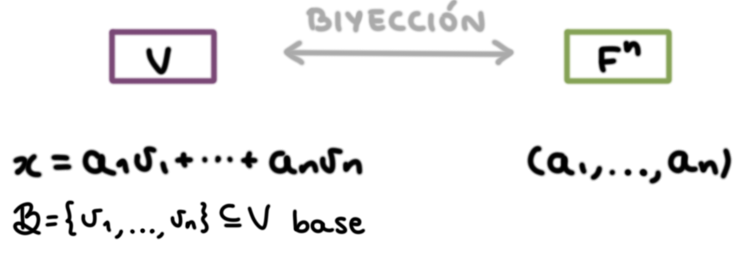
\includegraphics[scale = 3]{4} 
\end{figure}	

\begin{lema}
	\label{lema: S union x es ld sii x en generado de S}
Sean $S$ un subconjunto l.i. de $V$, $x \in V - S$.
Entonces, $S \cup \{ x \}$ es linealmente dependiente si y sólo
si $x \in \langle S \rangle$.
\end{lema}
\noindent
\textbf{Demostración.}
\begin{itemize}
	\item[$\Rightarrow$)] Suponiendo que $x$ no está en el generado por
	$S$, mostremos que $S \cup \{ x \} $ es l.i. o, equivalentemente,
	que todo subconjunto finito de él lo es. Sea 
	$\{ x_{1}, \ldots , x_{n-1} \} \cup \{ x \}$
	un subconjunto finito de $S \cup \{ x \}$ (¿por qué sólo interesa
	el caso en el que el subconjuto contiene a $x$?). Sean 
	$a_{i}$ escalares tales que 
	\[
	a_{1} x_{1} + \cdots + a_{n-1}x_{n-1} + a_{n}x = \hat{0}.
	\]
	Si $a_{n}$ fuese distinto de cero, despejando tendríamos que
	\[
	x = -\frac{a_{1}}{a_{n}}x_{1} + \cdots + -\frac{a_{n-1}}{a_{n}}x_{n-1}
	\in \langle S \rangle \hspace{0.5cm} \lightning
	\]
	Así, $a_{n} = 0$. Luego,
	\[
	a_{1} x_{1} + \cdots + a_{n-1}x_{n-1} = \hat{0}
	\]
	y, como $S$ es l.i., esto último implica la igualdad a cero 
	de todos los coeficientes.
	\item[$\Leftarrow$)] Puesto que
	\[
	x \in \langle S \rangle = \langle (S \cup \{ x \}) - \{ x \} \rangle,
	\]
	según la proposición \ref{prop: ld equiv fried y hugo},
	$S \cup \{ x \}$ es l.d..
\end{itemize}

\QEDB
\vspace{0.2cm}

\begin{teo}
	\label{teo: extrayendo bases de generadores finitos}
\marginnote{El teorema consiste en extrar bases de conjuntos
generadores finitos.} Si un espacio vectorial $V$ es generado
por un conjunto finito $S_{0}$, entonces un subconjunto de $S_{0}$
es base para $V$.
\end{teo}
\noindent
\textbf{Demostración.}
Si $S_{0} = \emptyset, \{ 0 \}$, entonces $V = \{ 0 \}$, y en ambos
casos puede extrarse del conjunto generador $S_{0}$ al vacío,
que es una base del espacio.

Supongamos ahora que $V \neq \{ 0 \}$ o, equivalentemente, que
$S_{0}$ contiene al menos un vector no cero $x_{1}$. Según el ejercicio
REF, $\{ x_{1} \}$ es linealmente independiente. Continue
escogiendo vectores $x_{2}, \ldots , x_{n} \in S_{0}$
tales que $S = \{ x_{1}, \ldots , x_{n} \}$ sigue siendo 
linealmente independiente y 
\begin{equation}
	\label{eq: 0, 28 ag}
	x \in S_{0} - S \Rightarrow S \cup \{ x \}
	\hspace{0.2cm} \textit{ es l.d.. }
\end{equation}
Según el lema 
\ref{lema: S union x es ld sii x en generado de S}, 
esto puede hacerse escogiendo
$x_{i} \in (V - \langle \{ x_{1}, \ldots , x_{i-1} \}) \cap S_{0}$.
\begin{figure}[H]
	\sidecaption{
	Figura que ilustra el proceso para la colección de cuatro
	vectores de $\IR^{3}$ que se muestra en el diagrama.
	\label{fig: 5}
	}
	\centering
	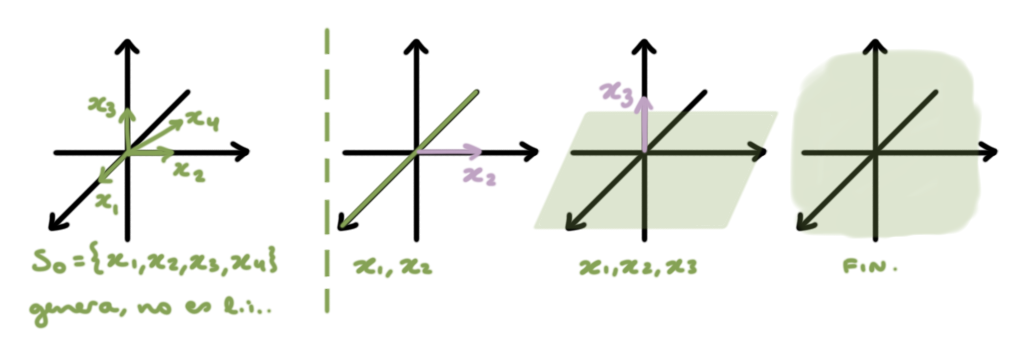
\includegraphics[scale = 2.8]{5} 
\end{figure}	
Como $S$ es finito, este proceso en efecto debe acabar,
es decir, no podemos ampliar indefinidamente a nuestro subconjunto
l.i. de $S_{0}$.

Aformamos que el l.i. $S$ es base del espacio $V$. Para demostrar esto,
bastará ver que $S_{0} \subseteq \langle S \rangle$
pues, en ese caso,
\[
V = \langle S_{0} \rangle \leq \langle \langle S \rangle \rangle
= \langle S \rangle \leq V. 
\]
Sea pues $x \in S_{0}$. Si $x \in S$, claramente 
$x \in \langle S \rangle$. En caso contrario, según 
\ref{eq: 0, 28 ag}, $S \cup \{ x \}$ es l.d., luego,
por el lema \ref{lema: S union x es ld sii x en generado de S},
$x \in \langle S \rangle$.
\QEDB
\vspace{0.2cm}

\begin{cor}
Si un espacio vectorial tiene un subconjunto finito que lo genera,
entonces tiene base (finita).
\end{cor}

La ventaja de la demostración del teorema
\ref{teo: extrayendo bases de generadores finitos}
es que es \textit{constructiva}, es decir, no sólo
muestra la existencia de tales bases, sino que explica
cómo construirlas.

Nota que hasta el momento no hemos dicho nada sobre la existencia
de bases en un espacio vectorial; nos vamos a limitar en esta
sección a hacer inferencias sobre espacios vectoriales que,
por hipótesis, tengan bases. 

\begin{teo}
	\label{teo: un li se completa a generador mediante una base}
\begin{marginfigure}
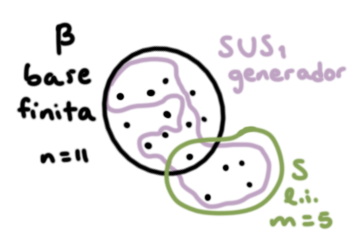
\includegraphics[scale= 3]{7} 
\end{marginfigure}
Sean $V$ un $F-$espacio vectorial, $\beta$ una base $V$ con $n$
elementos, $n \in \IN$. Sea
$S = \{ y_{1}, \ldots , y_{m} \}$ un subconjunto linealmente independiente
con $m \leq n$. Entonces, existe $S_{1}$ subconjunto de $\beta$
con $n-m$ elementos tal que $\langle S \cup S_{1} \rangle = V$.
\end{teo}
\noindent
\textbf{Demostración.}
Vamos a proceder por inducción sobre $m \leq n$.

\begin{figure}[H]
\centering\captionsetup{format = hang}
	\begin{measuredfigure}
		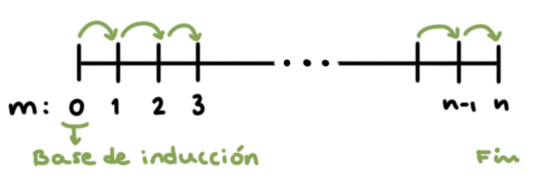
\includegraphics[scale=3]{6} 
 	\end{measuredfigure}
 \end{figure}
\begin{itemize}
\item \textit{Base de inducción:} si $m = 0$, o sea, si $S = \emptyset$,
entonces $S_{1} = \beta$ funciona.
\item \textit{Paso inductivo:} supongamos el teorema cierto para 
$m < n$ y demostremos que el teorema también se cumple para
$m+1$. Sea pues $S = \{ y_{1}, \ldots , y_{m}, y_{m+1} \}$
un subconjunto l.i. de $m+1$ elementos. 
\begin{marginfigure}
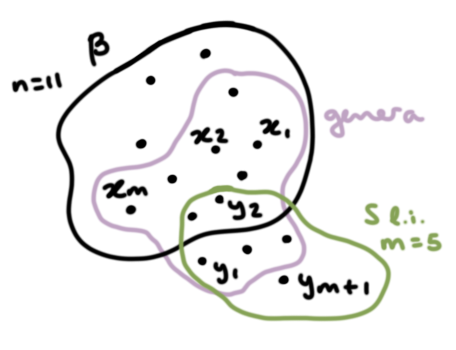
\includegraphics[scale=2.3]{8} 
\end{marginfigure}
Como $\{ y_{1}, \ldots y_{m} \}$ es un l.i. de $m$ elementos, por
hipótesis de inducción existe 
$\{ x_{1}, \ldots , x_{n-m} \} \subseteq \beta$ tal que 
\begin{equation}
	\label{eq: 0 29 Ag 24}
	\langle \{ y_{1}, \ldots , x_{m} \} \cup
	\{ x_{1}, \ldots , x_{n-m} \} \rangle = V.
\end{equation}
Existen pues escalares $a_{i}, b_{j} \in F$
tales que
\[
y_{m+1} = a_{1}y_{1} + \cdots + a_{m}y_{m} + 
b_{1}x_{1} + \cdots + b_{n-m}x_{n-m}.
\] 
Como $S$ es l.i., $y_{m+1}$ no puede ponerse como combinación
lineal de otros elementos de $S$, luego, al menos
algún $b_{j}$ debe no ser cero; sin pérdida de generalidad,
digamos que $b_{1} \neq 0$. Entonces, podemos despejar a 
$x_{1}$ de la ecuación anterior y llegar a que 
\[
x_{1} \in \langle \{ y_{1}, \ldots , y_{m+1} \} \cup
\{ x_{2}, \ldots , x_{n-m} \} \rangle;
\]
de esto se sigue que 
\begin{marginfigure}
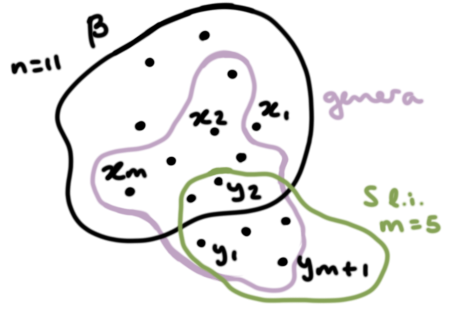
\includegraphics[scale=2.3]{9} 
\end{marginfigure}
\[
\{ y_{1}, \ldots , y_{m}, x_{1}, x_{2}, \ldots , x_{n-m} \}
\subseteq 
\langle
y_{1}, \ldots , y_{m}, y_{m+1}, x_{2}, \ldots, x_{n-m}
\rangle.
\]
Tomando generados a ambos lados de la igualdad y usando 
\eqref{eq: 0 29 Ag 24}, llegamos a que 
el subconjunto $\{x_{2}, \ldots , x_{n-m} \}$ de
$n-(m+1)$ elementos de $\beta$ es tal que 
\[
\langle
\{ y_{1}, \ldots , y_{m+1} \} \cup
\{ x_{2}, \ldots , x_{n-m} \}
\rangle = V.
\]
\end{itemize}
\QEDB
\vspace{0.2cm}

\begin{cor}
	\label{cor: li con n element es base}
Sea $V$ un $F-$espacio vectorial que tiene una base
$\beta$ con $n$ elementos. Entonces, cualquier subconjunto
l.i. de $V$ con $n$ elemenos es base de $V$. 
\end{cor}
\noindent
\textbf{Demostración.}
Según el teorema 
\ref{teo: un li se completa a generador mediante una base},
si $S$ es un tal subconjunto l.i., entonces existe $S_{1} \subseteq \beta$
tal que $S \cup S_{1}$ genera a $V$ y $S_{1}$ tiene
$n-n=0$ elementos; entonces, tal $S_{1}$ debe ser el vacío,
y $S = S \cup \emptyset$, además de ser l.i., genera a $V$,
luego, es base del espacio.

\QEDB
\vspace{0.2cm}

\begin{ejem}
En los ejercicios mostraste que $\IR^{3}$ tiene a 
$\{ (1, 0, 0), (0, 1, 0), (0, 0, 1) \}$ como base. Sean
los vectores 
$x_{1} = (1, -3, 2)$,
$x_{2} = (4, 1, 0)$ y $x_{3} = (0, 2, -1)$. Es fácil ver que
estos son linealmente independientes. Según el corolario
\ref{cor: li con n element es base}, esto implica que
ellos conforman una base para $\IR^{3}$.
\end{ejem}

\marginnote{Este Corolario nos indica que la cardinalidad de una
base finita de $V$ acota la cardinalidad de los subconjuntos
l.i. del espacio.}
\begin{cor}
	\label{cor: cardinalidad de bases limita la de los li}
Sea $V$ un $F-$espacio vectorial. Si existe $\beta$ base de
$V$ con $n$ elementos, entonces cualquier subconjunto de $V$
con más de $n$ elementos es l.d..
\end{cor}
\noindent
\textbf{Demostración.}
Sea $S \subseteq V$ con $|S| > n$. Supongamos que $S$ es l.i..
Si $S_{1}$ es un subconjunto de $S$ con al menos $n$ elementos, 
entonces al igual que $S$ es l.i., luego, por el corolario 
\ref{cor: li con n element es base} es una base del espacio,
entonces,  $\langle S_{1} \rangle = V$.
Si $x \in S - S_{1}$, como $x \in V = \langle S_{1} \rangle$,
por el lema 
\ref{lema: S union x es ld sii x en generado de S},
$S_{1} \cup \{ x \} \subseteq S$ es l.d., luego,
$S$ es l.d.  $\lightning$

\QEDB
\vspace{0.2cm}

\begin{cor}
Sea $V$ un $F-$espacio vectorial. Si existe 
$\beta \subseteq V$ base de $n$ elementos, entonces
cualquier otra base de $V$ tendrá $n$ elementos.
\end{cor}
\noindent
\textbf{Demostración.}
Sea $\gamma \subseteq V$ otra base de $V$.
Como $\gamma$ (respectivamente, $\beta$) es linealmente independiente
y $\beta$ (respectivamente, $\gamma$) es base del espacio,
por el corolario 
\ref{cor: cardinalidad de bases limita la de los li}
$|\gamma| \leq |\beta|$ (respectivamente, 
$|\beta| \leq |\gamma|$).

\QEDB
\vspace{0.2cm}

Este último resultado nos permite introducir la noción 
de dimensión.

\begin{defi}
Un espacio vectorial se dice \textbf{finito dimensional}
si tiene una base que consta de un número finito de elementos.
El único número de elementos en cada base del espacio se llama
la \textbf{dimensión de $V$}, y se denotará por
$dim(V)$. Todo espacio vectorial que no sea finito dimensional
será llamado \textbf{infinito dimensional}.
\end{defi}

Nota que hasta el momento hemos encontrado resultados válidos
para cuando el espacio vectorial tiene una base finita; aunque 
con lo visto hasta ahora no podemos asegurar que cualquier
espacio vectorial tiene base, esto es cierto y puede
demostrarse usando el Lema de Zorn. Puedes consultar los
detalles en Friedberg, sección 1.7.
En la práctica, casi siempre se usarán espacios de dimensión
finita (de hecho, algún $\IR^{n}$).


\begin{ejem}
Demuestre las siguientes afirmaciones:
\begin{itemize}
	\item El espacio vectorial $\{ 0 \}$ tiene dimensión cero.
	\item El espacio vectorial $F^{n}$ tiene dimensión $n$.
	\item El espacio vectorial $M_{m \times n} (F)$ tiene dimensión
	$m \times n$.
	\item El espacio vectorial $P_{n}(F)$ tiene dimensión
	$n+1$.
	\item El espacio vectorial $P(F)$ es infinito dimensional.
\end{itemize}
\end{ejem}


\begin{ejem}
Ilustramos a continuación el que la dimensión de un
$F-$espacio vectorial $V$ depende no solo del grupo abeliano $V$,
sino también del campo $F$.
\begin{itemize}
	\item El $\IC-$ espacio vectorial $\IC$ tiene dimensión $1$.
	En efecto, $\{ 1 \}$ es base para él, pues
	\begin{itemize}
		\item el singulete $\{ 1 \}$ es l.i., y,
		\item dado $z \in \IC$, $z = 1 \cdot z \in \langle \{ 1 \} \rangle$,
		luego, $\langle \{ 1 \} = \IC$.
	\end{itemize}
	\item El $\IR-$espacio vectorial $\IC$ tiene dimensión $2$,
	pues una base de este espacio es $\{ 1, i \}$;
	\begin{itemize}
		\item Dado $z = a + b i \in \IC$ (donde $a, b \in \IR$),
		$z = a \cdot 1 + b \cdot i \in \langle \{ 1, i \} \rangle$, y
		\item no existe $a \in \IR$ tal que $a \cdot 1 = i$, luego,
		$i$ no es múltiplo escalar de $1$, por lo que 
		$\{ 1, i \}$ es l.i..
	\end{itemize}
\end{itemize}
\end{ejem}

\begin{cor}
	\label{cor: generador de n elementos es base en un n dim}
Sea $V$ un $F-$espacio vectorial de dimensión $n$. Si
$S \subseteq V$ genera a $V$ y tiene a lo más $n$ elementos, entonces $S$
es base de $V$ (luego, $|S| = n$).
\end{cor}
\noindent
\textbf{Demostración.}
Por el teorema 
\ref{teo: extrayendo bases de generadores finitos}, 
sabemos que existe $S_{1} \subseteq S$ base de $V$.
Entonces, como $V$ es $n-$dimensional,
$|S_{1}| = n$; entonces, $|S| \leq n$ y $S$ tiene 
un subconjunto $S_{1}$ de $n$ elementos, luego $S$ tiene $n$
elementos y coincide con $S_{1}$, 
por lo tanto, es base de $V$.
\QEDB
\vspace{0.2cm}

\begin{figure}[H]
	\sidecaption{
	Según lo estudiado ahora, la cardinalidad de un 
	subconjunto de un espacio vectorial $n-$dimensional
	nos indica si puede o no ser l.i. o generador.
	}
	\centering
	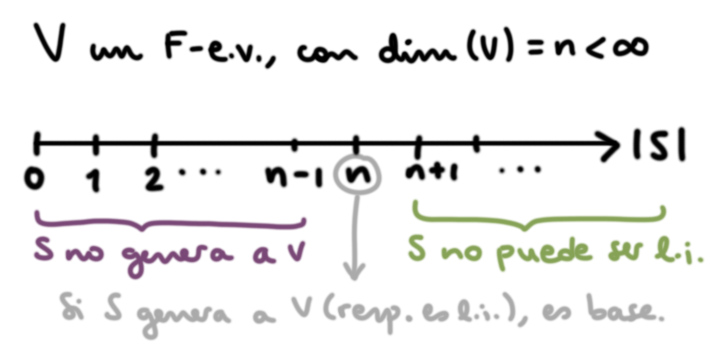
\includegraphics[scale = 3]{10} 
\end{figure}	

\begin{cor}
	\label{cor: extendiendo l.i. a base finita}
\marginnote{Este corolario nos explica cómo extender l.i.'s a 
bases finitas.}
Sea $\beta$ una base de un espacio vectorial $V$ de dimensión
$n$. Sea $S \subseteq V$ linealmente independiente. Existe
$S_{1} \subseteq \beta$ tal que $S \cup S_{1}$ es base de $V$.
\end{cor}
\noindent
\textbf{Demostración.}
Por el corolario \ref{cor: cardinalidad de bases limita la de los li},
$m := |S| \leq n$, entonces, por el teorema 
\ref{teo: un li se completa a generador mediante una base},
existe $S_{1} \subseteq \beta$ con 
$|S_{1}| = n-m$ tal que $S \cup S_{1}$ genera a $V$.
Claro que $|S \cup S_{1}| \leq n$; así, por el corolario 
\ref{cor: generador de n elementos es base en un n dim}, 
$S \cup S_{1}$ es base de $V$.
\QEDB
\vspace{0.2cm}

Resumimos lo deducido hasta ahora:
\begin{itemize}
	\item Una base de un espacio vectorial es un subconjunto de este
	que lo genera y es linealmente independiente.
	\item Si $V$ tiene una base finita, entonces cualquier base de $V$
	tiene el mismo número de vectores. A este número $n$ se le llama la 
	dimensión de $V$.
	\begin{marginfigure}
		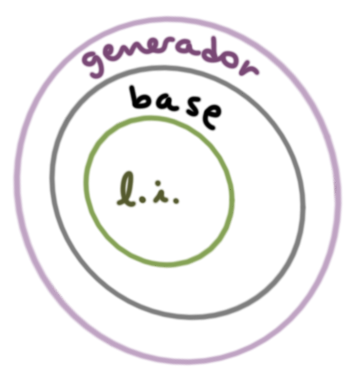
\includegraphics[scale= 2.5]{11}
	\end{marginfigure}
	\item En este caso, todo subconjunto linealmente independiente
	o generador de $n$ elementos es base del espacio,
	\item todo subconjunto l.i. contiene a lo más $n$
	vectores (c.f. corolario
	\ref{cor: cardinalidad de bases limita la de los li}),
	y en caso de tener menos de $n$ vectores (i.e. en caso de no ser base)
	puede completarse a una base
	del espacio (c.f. corolario 
	\ref{cor: extendiendo l.i. a base finita}).
	\item Recíprocamente, si $dim(V) = n$, entonces todo subconjunto
	generador contiene por lo menos $n$ elementos
	y de él se puede extraer una base de $V$ eliminando vectores
	que hagan al generador redundante (recuerda este proceso explicado
	en la demostración del teorema 
	\ref{teo: extrayendo bases de generadores finitos}).

\end{itemize}

\hlpink{Agregar el proceso para extender un l.i. a una base de un
espacio finito dimensional con la ayuda del lema}
\ref{lema: S union x es ld sii x en generado de S}. Poner el ejemplo
práctico en $M_{2 \times 2}(\IR)$.

\section{Caso práctico: Interpolación con polinomios de Lagrange}


La situación es la siguiente: se tiene un conjunto de $n+1$ datos
\marginnote{Interpolación: 
obtención de nuevos puntos partiendo del conocimiento de un conjunto de puntos.}
\[
\{ (c_{0}, b_{0}), (c_{1}, b_{1}), \ldots , (c_{n}, b_{n}) \},
\]
con $c_{i} \neq c_{j}$ si $i \neq j$, y se requiere
hacer una interpolación de estos con un polinomio
del menor grado posible. 
\begin{itemize}
	\item Nos gustaría usar un polinomio, pues es una función
	con la que es muy fácil trabajar, tanto teórica
	como prácticamente.
	\item Además, no queremos que el grado sea alto 
	(relativo a la cantidad de datos) para evitar situaciones
	como las de la figura: el aumentar el grado del polinomio
	aumenta el número de ceros de este, luego, la cantidad de
	oscilaciones, por lo que usar un grado demasiado alto hace
	que, a pesar de que el polinomio coincida con los puntos
	$b_{i}$ en los valores $c_{i}$, no modele bien su patrón
	de comportamiento.
\end{itemize}

\begin{marginfigure}
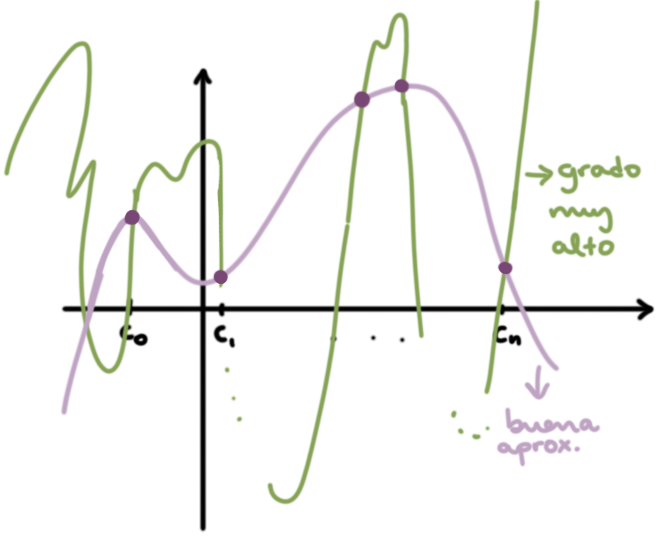
\includegraphics[scale= 1.8]{12} 
\end{marginfigure}

Para $0 \leq i \leq n$, definamos
\begin{equation}
	\label{eq: defi pol lagrange}
	f_{i}(x) := \frac{
	(x-c_{0}) (x-c_{1}) \cdots (x-c_{i-1})
	(x-c_{i+1}) \cdots (x-c_{n})
	}{(c_{i} - c_{0}) (c_{i}-c_{1}) \cdots
	(c_{i}-c_{i-1})(c_{i}-c_{i+1}) \cdots (c_{i}-c_{n}) }
	= \prod_{\substack{j=0 \\ j \neq i}}^{n} \frac{x-c_{j}}{c_{i}-c_{j}}.
\end{equation}
\marginnote{La condición \ref{eq: propiedad pol lagrange} es la que define
a los polinomios de Lagrange.}
A estos $n+1$ polinomios se les llama los
\textbf{polinomios de Lagrange asociados a $c_{0}, c_{1}, \ldots , c_{n}$}.
Por supuesto que
\begin{equation}
	\label{eq: propiedad pol lagrange}
	f_{i}(c_{j}) 
	= \begin{cases}
	0 & \textit{ si } j \neq i, \\
	1 & \textit{ si } j = i.
	\end{cases}
\end{equation}

\begin{figure}[H]
	\sidecaption{
	Polinomios de Lagrange asociados a la malla 
	$[-3, 0.8,  5, 9]$.
	}
	\centering
	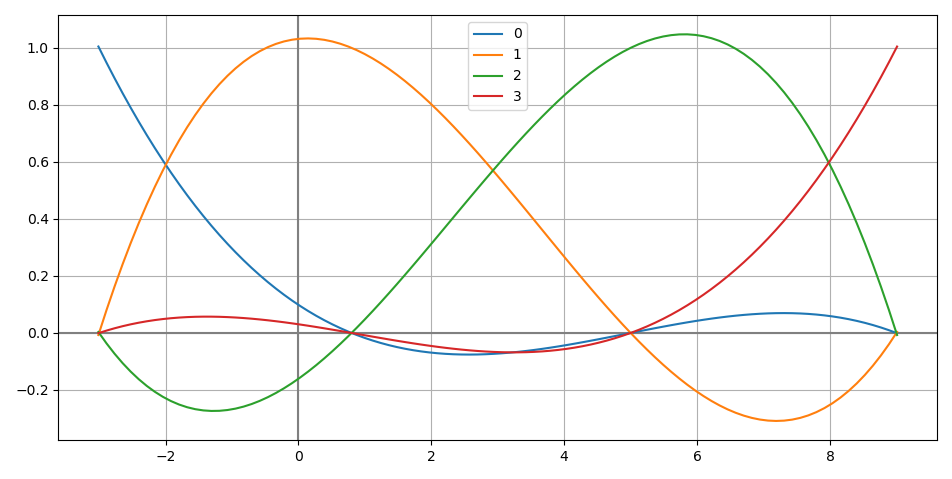
\includegraphics[scale = 0.5]{15} 
\end{figure}	



\begin{prop}
Sean $c_{0} < c_{1} < \cdots < c_{n}$ números reales. Si
$\beta = \{ f_{0}, \ldots, f_{n} \}$ es el conjunto de los
polinomios de Lagrange 
\eqref{eq: defi pol lagrange} asociados a estos números,
entonces $\beta$ es una base del $F$ espacio vectorial
$P_{n}(F)$.
\end{prop}
\noindent
\textbf{Demostración.}
Si demostramos que el conjunto de $n+1$ vectores 
$\beta$ es l.i. podremos concluir que es base de
$P_{n}(F)$ (¿por qué?).
Sean $a_{0}, a_{1}, \ldots, a_{n} \in F$ tales que
$a_{0}f_{0} + \cdots + a_{n}f_{n}$ es el polinomio ero.
Entonces, para toda $0 \leq j \leq n$,
usando la propiedad \eqref{eq: propiedad pol lagrange}
se tiene que 
\begin{align*}
0 = \hat{0}(c_{j}) = &
(a_{0}f_{0} + a_{1}f_{1} + \cdots + a_{n}f_{n})(c_{j}) \\
= & \sum_{i=1}^{n} a_{i}f_{i}(c_{j}) = a_{j} \cdot 1 = a_{j}.
\end{align*}

\QEDB
\vspace{0.2cm}


Así, dado $g \in P_{n}(F)$ cualquiera, existen únicos
$b_{i} \in F$ tales que $g = \sum_{i = 0}^{n}b_{i}f_{i}$;
de hecho, la propiedad \eqref{eq: propiedad pol lagrange}
nos permite dar explícitamente a tales coeficientes $b_{i}$;
para toda $0 \leq j \leq n$,
\[
g(c_{j}) = \left( \sum_{i = 0}^{n}b_{i}f_{i} \right)(c_{j})
= b_{j}.
\]
Así,
\begin{equation}
	\label{eq: g como comb lineal de los de lagrange}
	g = \sum_{i=0}^{n}g(c_{i})f_{i}.
	\hspace{0.2cm} \textit{(Ecuación de interpolación de Lagrange)}
\end{equation}


Regresando a la situación planteada al inicio,
dada la colección de datos 
$$\{ (c_{0}, b_{0}), (c_{1}, b_{1}), \ldots , (c_{n}, b_{n}) \},$$
el único polinomio $g$ de grado a lo más $n$ tal que
$g(c_{i}) = b_{i}$ para toda $i$ es 
\eqref{eq: g como comb lineal de los de lagrange}.

\begin{figure}[H]
	\sidecaption{
	Polinomio de interpolación de Lagrange para los datos
	$(-3,-1), (-2, 4), (-1, 2), (0, 0.8),$ 
	$(2, -0.5), (3, 0.6), (4, 1)$, 
	$(5, 3), (5.5, 3.5)$.
	\label{fig: interp}
	}
	\centering
	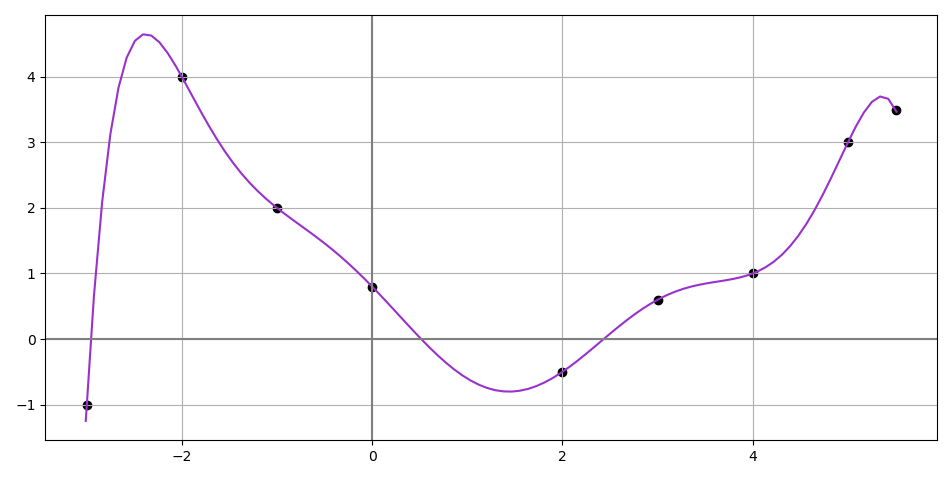
\includegraphics[scale = 0.5 ]{14} 
\end{figure}	




\section{Algunos resultados de dimensión}

\begin{teo}
	\label{teo: la dim de subespacios es menor o igual a la del espacio}
Sea $V$ un $F-$espacio vectorial de dimensión $n$.
Todo subespacio de $V$ será también finito dimensional, y
si dimensión será menor o igual a $n$; si es igual a $n$,
entonces coincide con todo el espacio $V$.
\end{teo}
\noindent
\textbf{Demostración.}
Sea $W \leq V$.
Si $W = \{ 0 \}$, entonces $dim(W) = 0 \leq n$. Supongamos ahora
que W tiene al menos un elemento no cero $x_{1}$.
El singulete
$\{ x_{1} \}$ es entonces l.i.
(c.f. proposición \ref{prop: singulete x l.i. sii x no cero}).
Podemos continuar de esta forma tomando elementos
$x_{1}, \ldots, x_{k}$ de $W$
tales que $\{ x_{1}, \ldots , x_{k} \}$ es l.i.
pero, adjuntando otro vector de $W$, se pierde la independencia
lineal (esto porque en $V$ no puede haber subconjuntos linealmente
independientes de más de elementos, luego, de hecho
ocurre $k \leq n$).
Según el lema 
\ref{lema: S union x es ld sii x en generado de S}, esto implica
que
\[
\forall x \in W - \{ x_{1}, \ldots , x_{k} \}:
\hspace{0.2cm} x \in \langle \{ x_{1}, \ldots , x_{k} \} \rangle,
\]
luego, 
\[
W = \langle \{ x_{1}, \ldots , x_{k} \} \rangle.
\]
Así, el l.i. $\{ x_{1}, \ldots , x_{k} \}$
genera a $W$, por lo tanto, es base de $W$.
Entonces, $dim (W) = k \leq n$.

Si ocurriese $dim(W) = n$, entonces una base $\beta$ de $W$
es un subconjunto l.i. de $V$ de $n = dim(V)$ elementos,
por lo tanto, es también una base de $V$
(c.f. corolario \ref{cor: li con n element es base}),
luego,
\[
W = \langle \beta \rangle = V.
\]
\QEDB
\vspace{0.2cm}

\begin{cor}
Si $V$ es finito dimensional, entonces toda base
$\beta$ de un subespacio de $W$ puede extenderse a una base de $V$.
\end{cor}
\noindent
\textbf{Demostración.}
Si $\beta$ es base de $W$, en particular es un subconjunto
l.i. de $V$, luego, según el corolario 
\ref{cor: extendiendo l.i. a base finita}, puede extenderse a una
base de $V$.
\QEDB
\vspace{0.2cm}

\begin{teo}
Si $W_{1}, W_{2}$ son dos subespacios de $V$ finito dimensionales,
entonces $W_{1} + W_{2}$ es también finito dimensional, y 
\[
dim(W_{1} + W_{2}) = dim(W_{1}) + dim(W_{2}) - dim(W_{1} \cap W_{2}).
\]
\end{teo}
\noindent
\textbf{Demostración.}
Note primero que $W_{1} \cap W_{2}$ es subespacio de un espacio
finito dimensional (por ejemplo, de $W_{1}$), luego, es también
finito dimensional. Sea pues
$\beta_{0} = \{ x_{1}, \ldots , x_{k} \}$ base de 
$W_{1} \cap W_{2}$, y sean 
$\beta_{1} = \{ y_{1}, \ldots , y_{r} \}$, 
$\beta_{2} = \{ z_{1}, \ldots , z_{m} \}$
tales que
\[
\beta_{0} \cup \beta_{i} \hspace{0.5cm}
\textit{ es base de } W_{i}, \hspace{0.1cm} i = 1,2.
\] 
\begin{itemize}
	\item Veamos que $\beta_{0} \cup \beta_{1} \cup \beta_{2}$
	es l.i.. Sea escalares $a_{i}$, $b_{j}$ y $c_{l}$ tales que 
	\begin{equation}
		\label{eq: 1, 5 sept 24}
		a_{1}x_{1} + \cdots + a_{k} x_{k} + 
		b_{1}y_{1} + \cdots b_{r}y_{r} +
		c_{1}z_{1} + \cdots + c_{m}z_{m} = \hat{0}.
	\end{equation}
	Definiendo
	\[
	v_{0} = a_{1}x_{1} + \cdots + a_{k} x_{k},
	\hspace{0.1cm}
	v_{1} = b_{1}y_{1} + \cdots b_{r}y_{r},
	\hspace{0.1cm}
	v_{2} = c_{1}z_{1} + \cdots + c_{m}z_{m},
	\]
	la ecuación \eqref{eq: 1, 5 sept 24}
	se reescribe como
	\[
	v_{0} + v_{1} + v_{2} = \hat{0}.
	\]
	Por supuesto que $v_{0} \in W_{1} \cap W_{2}$,
	$v_{1}  \in W_{1}$, $v_{2} \in W_{2}$.
	Despejando a $v_{2}$ de esta última ecuación, se tiene que
	$v_{2} = v_{0} + v_{1} \in W_{1}$, luego,
	$v_{2} \in W_{1} \cap W_{2}$.
	Puesto que $\beta_{0}$ es base de este espacio, existen
	escalares $d_{i}$ tales que 
	\begin{equation}
		\label{eq: 2, 5 sept 24}
		v_{2} = d_{1}x_{1} + \cdots + d_{n} x_{n};
	\end{equation}
	sustituyendo en \eqref{eq: 1, 5 sept 24}, se llega a que
	\[
	(a_{1}+d_{1})x_{1} + \cdots + (a_{k}+d_{k})x_{k} +
	b_{1}y_{1} + \cdots + b_{k}y_{k} = \hat{0};
	\]
	la independencia lineal de $\beta_{0}\cup \beta_{1}$
	implica que todos los escalares de la combinación lineal
	anterior son cero, en particular, que 
	$b_{1} = \cdots = b_{k} = 0$. Sustituyendo esto en 
	\eqref{eq: 1, 5 sept 24}, se tiene que 
	\[
	(a_{1})x_{1} + \cdots + (a_{k})x_{k} +
	c_{1}z_{1} + \cdots + c_{m}z_{m} = \hat{0}.
	\]
	Ahora la independencia lineal de $\beta_{0} \cup \beta_{2}$
	nos permite concluir que también los escalares $a_{i}$ y
	$c_{l}$ son todos cero.
	
	Con esto demostramos la independencia lineal de 
	$\beta_{0} \cup \beta_{1} \cup \beta_{2}$. Nota que esto
	implica que $\beta_{0}$, $\beta_{1}$ y
	$\beta_{2}$ son ajenos dos a dos, luego,
	\begin{equation}
		\label{eq: cardinalidad de base de w1 mas w2}
		|\beta_{0} \cup \beta_{1} \cup \beta_{2}| = k + r + m.
	\end{equation}
	
	\item Mostremos que
	\marginnote{Es fácil comprobar que, para cualesquiera subconjuntos
	$A, B \subseteq V$, 
	\[
	\langle A \cup B \rangle = \langle A \rangle + 
	\langle B \rangle.
	\]}	
	 $\beta_{0} \cup \beta_{1} \cup \beta_{2}$
	genera a $W_{1} + W_{2}$;
	\begin{align*}
	\langle \beta_{0} \cup \beta_{1} \cup \beta_{2} \rangle
	= & \langle
	( \beta_{0} \cup \beta_{1} ) \cup 
	( \beta_{0} \cup \beta_{2} )
	\rangle \\
	= & \langle  \beta_{0} \cup \beta_{1}  \rangle + 
	\langle  \beta_{0} \cup \beta_{2} \rangle \\
	= & W_{1} + W_{2}. 
	\end{align*}
	
	Hemos demostrado así que 
	$\beta_{0} \cup \beta_{1} \cup \beta_{2}$
	es base de $W_{1} + W_{2}$; de esto y 
	\eqref{eq: cardinalidad de base de w1 mas w2}
	se concluye que 
	\begin{align*}
	dim(W_{1} + W_{1}) = k + r + m = &
	(k+r) + (k+m) - k \\
	= & dim(W_{1}) + dim(W_{2}) - dim(W_{1} \cap W_{2}).
	\end{align*}
\end{itemize}
\QEDB
\vspace{0.2cm}

De este teorema y de la proposición 
\ref{prop: suma directa sii interseccion cero}
se sigue el siguiente

\begin{cor}
Si $W_{1}$ y $W_{2}$ son subespacios de $V$ finito dimensionales,
entonces la suma $W_{1} + W_{2}$ es directa si y sólo si 
\[
dim(W_{1} + W_{2}) = dim(W_{1}) + dim(W_{2}).
\]
\end{cor}


\begin{ejem}
Si $U, V$ son dos subespacios de $\IR^{9}$ ambos de dimensión $5$,
entonces su suma no puede ser directa, pues
\[
9 \geq dim(U + V) = dim(U) + dim(V) - dim(U \cap V) = 10 - dim(U \cap V),
\]
luego, $dim(U \cap V) \geq 1$, por lo que no puede ocurrir
$U \cap V = \{ 0 \}$.
\end{ejem}

\begin{ejem}
Considere al $\IR$ espacio vectorial $P_{4}(\IR)$ de los polinomios
con coeficientes reales y grado no mayor a cuatro.
Sea
\[
U = \{ f \in P_{4}(\IR)  | \hspace{0.2cm} f(6) = 0 \}
\]
el conjunto de los polinomios de grado a lo más cuatro que tienen al
$6$ como raíz. Claro que $U$ es un subespacio
(propia) de $P_{4}(\IR)$,
pues
\begin{itemize}
	\item El polinomio cero tiene a $6$ como raíz,
	\item Si $f, g \in U$ y $a \in \IR$, entonces $6$ es raíz del polinomio
	$af + g$, pues $(af+g)(6) = a \cdot f(6) + g(6) = a \cdot 0 + 0 = 0$.
\end{itemize}
Según el teorema \ref{teo: la dim de subespacios es menor o igual a la del espacio},
$0 \leq dim(U) \leq 4$ (pues $dim(P_{4}) = 5$).
Observe que los cuatro polinomios
\[
f_{i}(x) := (x-6)^{i}, \hspace{0.2cm}
1 \leq i \leq 4
\]
son todos elementos de $U$, y además son linealmente independientes
(sus grados son todos distintos entre sí), luego,
ellos conforman una base para el espacio, y $dim(U) = 4$.

\begin{marginfigure}
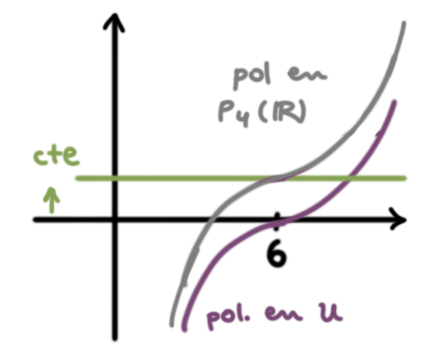
\includegraphics[scale=2]{13} 
		\caption{Todo polinomio en $P_{4}(\IR)$ se
expresa de forma única como la suma de un polinomio en $U$ y 
uno constante.}
\end{marginfigure}

Una base de $P_{4}(\IR)$ que contiene a esta base de $U$ es
\[
\beta = \{ 1, f_{1}, f_{2}, f_{3}, f_{4} \}.
\]
Nota que el subespacio
\[
W = \{ f \in P_{4}(\IR)  | \hspace{0.2cm} f \textit{ es un
polinomio constante o el polinomio cero} \}
\]
es tal que $P_{4}(\IR) = U \oplus W$, pues
$U \cap W = \{ 0 \}$ - el único elemento de $W$ que tiene
a $6$ como raíz es el polinomio cero (de hecho, todo número
real es raíz del polinomio cero, no hay nada especial en el número
$6$ tomado para este ejemplo).
\end{ejem}

Terminemos con unos comentarios más sobre el concepto de dimensión:
es muy importante no confundir la noción de dimensión con
la de cardinalidad: por ejemplo, en $\IR^{3}$, 
\begin{itemize}
	\item toda recta que pasa por el origen es un subespacio
	de dimensión uno, y su cardinalidad $|\IR|$, 
	\item todo plano que pasa por el origen es un subespacio
	de dimensión dos, y su cardinalidad es $|\IR \times \IR| = |\IR|$.
\end{itemize}
Nótese que la dimensión parece ser un mejor indicador del
``tamaño'' de un subespacio, no la cardinalidad de este. 
\newpage









































